%%%%%%%%%%%%%%%%%%%%%%%%
% $Autor: MansourAhmadyPhoulady, RanjeetsingTawar, HemanthPrabhakaran$
% $Pfad: Car_Licence_Plate_Identification_with_a_JetsonNano$
% $Version: 4.0.0 $
%
% !TeX encoding = utf8
%
%%%%%%%%%%%%%%%%%%%%%%%%
\chapter{KDD Process - Knowledge Discovery in Databases Process}

	
	%\GRAPHICSC{1.0}{1.0}{BigData/KDD}
	%\begin{tikzpicture}[scale=0.8]
		
	%	\draw[black,fill=black!50] (-1,-4) -- (16,-4) -- (16,6) -- (-1,6) -- cycle;
	%	\node (Do) at (7.5,5.5) {\textcolor{white}{\textbf{Domain - Problem}}};
		
	%	\draw[draw, black!80, fill=black!10]  (-0.5,2) rectangle (15.5,5.1);
		
	%	\node[right] at (-0.1,4.6) {\textbf{Deployment}};
		
	%	\draw[draw, black!80, fill=black!5]  (-0.5,-3.5) rectangle (15.5,1.5);
		
	%	\node[right] at (-0.1,-3) {\textbf{Development}};
		
		
	%	\draw[draw, black!80, fill=blue!20!red!20]  (0.10,3.10) rectangle (3.10,4.20);
	%	\draw[draw, black!80, fill=blue!20!red!20]  (0.05,3.05) rectangle (3.05,4.15);
	%	\draw[draw, black!80, fill=blue!20!red!20]  (0,3) rectangle (3,4.1);
	%	\node (AMP) at (1.5,3.55) {\footnotesize Databases};
		
		%\visible<2->
	%	{
	%		\draw[->] (1.5,3)--(1.5,1.1);
	%		\draw[draw, black!80, fill=blue!20]  (0,0) rectangle (3,1.1);
	%		\node (AMP) at (1.5,0.75) {\footnotesize Data};
	%		\node (AMP) at (1.5,0.25) {\footnotesize Selection};
	%	}
		
		%\visible<3->
	%	{
	%		\draw[->] (3,0.55)--(3.5,0.55);
	%		\draw[draw, black!80, fill=blue!20]  (3.5,0) rectangle (6,1.1);
	%		\node (AMP) at (4.75,0.75) {\footnotesize Data};
	%		\node (AMP) at (4.75,0.25) {\footnotesize Preparation};
	%	}
		
		
		%\visible<4->
	%	{
	%		\draw[->] (6,0.55)--(6.5,0.55);
	%		\draw[draw, black!80, fill=blue!20]  (6.5,0) rectangle (9,1.1);
	%		\node (AMP) at (7.75,0.75) {\footnotesize Data Trans-};
	%		\node (AMP) at (7.75,0.25) {\footnotesize formation};
	%	}
		
		%\visible<5->
	%	{
	%		\draw[->] (9.0,0.55)--(9.5,0.55);
	%		\draw[draw, black!80, fill=green!20]  (9.5,0) rectangle (12,1.1);
	%		\node (AMP) at (10.75,0.75) {\footnotesize Data};
	%		\node (AMP) at (10.75,0.25) {\footnotesize Mining};
	%	}
		
		%\visible<6->
	%	{
	%		\draw[->] (10.75,1.1)--(10.75,3);
	%		\draw[draw, black!80, fill=yellow!20]  (9.5,3) rectangle (12,4.1);
	%		\node (AMP) at (10.75,3.75) {\footnotesize Model,};
	%		\node (AMP) at (10.75,3.25) {\footnotesize Patterns};
	%	}
		
	%	{
	%		\draw[->] (9,3.55)--(9.5,3.55);
	%		\draw[draw, black!80, fill=yellow!20]  (6.5,3) rectangle (9,4.1);
	%		\node (AMP) at (7.75,3.55) {\footnotesize New Data};
		
	%}
		
		%{
		%	\draw[->] (12,3.55)--(12.5,3.55);
		%	\draw[draw, black!80, fill=yellow!20]  (12.5,3) rectangle (15,4.1);
		%	\node (AMP) at (13.75,3.55) {\footnotesize Results};
		%}
		
		%\visible<7->
		%{
			%\draw[->] (10.75,0)--(10.75,-1.7);
			%\draw[draw, black!80, fill=blue!20]  (9.5,-2.8) rectangle %(12,-1.7);
%			\node (AMP) at (10.75,-2.05) {\footnotesize Evaluation,};
%			\node (AMP) at (10.75,-2.55) {\footnotesize Verification};
%		}
		
		%\visible<8->
%		{
%			\draw[-] (9.5,-2.25) -- (1.5,-2.25);
%			\draw[->] (1.5,-2.25)--(1.5,0);
%		}
		
		%\visible<9->
%		{
%			\draw[->] (4.75,-2.25)--(4.75,0);
%			\draw[->] (7.75,-2.25)--(7.75,0);
%		}
		
		%\visible<2->
%		{
%			\draw[red, thick, dash dot,-] (13.75,3)--(13.75,-2.2);
%			\draw[red,thick, dash dot,->] (13.75,-2.25) -- (12,-2.25);
			
%			\draw[red,thick, dash dot,->] (6.5,3.55) -- (3,3.55);
%		}
%	\end{tikzpicture}
%	\captionof{figure}{\textbf{KDDProcess Workflow}}
%\end{center}
\begin{figure}
	\centering
	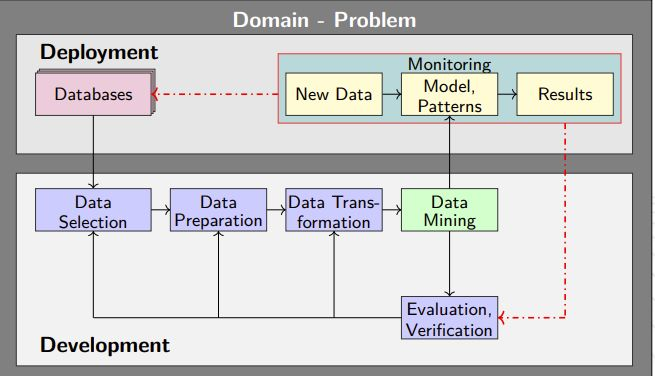
\includegraphics[width=\textwidth]{Images/KDDMonitoring}
	\caption{KDDProcess flow} \cite{Wings23}
	\label{fig:kdd}
\end{figure}

\section{Why KDD for Car License Plate Detection with Jetson Nano?}

The KDD process proves to be an optimal and systematic approach for the Car License Plate Detection project, especially given its comprehensive methodology designed to extract valuable insights from intricate datasets. In the realm of Car License Plate Detection, where the data encompasses diverse information from sensors capturing nuanced details, the initial phase of data exploration and understanding holds utmost importance. The KDD methodology's emphasis on iterative processes seamlessly aligns with the project's evolving nature, enabling continuous refinement and improvement based on insights gained from each iteration . Feature engineering for license plate data requires careful consideration to extract pertinent information for model training. KDD's structured approach addresses this need by prioritizing feature selection and extraction. Furthermore, the KDD process includes crucial steps such as data cleaning and preprocessing, tackling challenges like noise, outliers, and missing values. These steps are essential for ensuring the accuracy and reliability of the license plate detection model \\


KDD is an important step in the knowledge discovery process. Data mining is the process of extracting interesting patterns from large amounts of data. You can get a solution to your problem by analyzing the data that is already  in the dataset. It automatically learns from historical data and provides tools for building models for predicting future trends and behaviors. The essence of data mining is an important process for identifying valid, novel, potentially useful, and ultimately understandable patterns in your data.\\

In general, data mining tasks can be divided into two categories: descriptive tasks and predictive tasks. A descriptive data mining model can  extract useful patterns that describe the extracted data, examine its properties, and attempt to characterize the general properties of the data in the database. Predictive mining tasks draw conclusions and make predictions based on  current data.it attempts to predict unknown or future trends and behavior, depending on other variables or historical values displayed in the retrieved database.
Data mining is  used by a variety of companies and organizations, especially in the fields of medicine, retail, marketing, finance, telecommunications, and science. This provides these companies with information about their illness, sales behavior, customer satisfaction, and  interests. With the help of data mining, organizations can increase the profitability of patient-customer interactions and improve marketing risk management. The patterns extracted using data mining help businesses make better decisions. The following sections describe various data mining tasks.


\begin{enumerate}
	
	\item \textbf{Domain - Problem}: The domain problem in the KDD process refers to the identification and understanding of the problem domain that the data mining project aims to address. This involves defining the scope of the problem, specifying the relevant data sources, and understanding the domain-specific constraints, assumptions, and requirements.
	
	\item \textbf{Development}
	
	\begin{itemize}
		\item \textbf{Data Selection}: This is the initial stage of the KDD process where the relevant data is selected from the available sources. This may involve selecting data from multiple sources, merging datasets, or sampling to reduce the size of the dataset.
		
		\item \textbf{Data Preparation}: In this stage, the selected data is cleaned and preprocessed to ensure consistency and improve the quality of the data. This may include tasks such as data cleaning, filling missing values, handling outliers, and transforming data into appropriate formats.
		
		\item \textbf{Data Transformation}: The preprocessed data is then transformed into a suitable format for data mining. This stage may involve selecting appropriate attributes or features, normalizing data, and reducing the dimensionality of the dataset.
		
		\item \textbf{Data Mining}: This is the core stage of the KDD process where various data mining techniques such as clustering, classification, association rule mining, and outlier detection are applied to extract useful patterns and insights from the data.
		
		\item \textbf{Evaluation, Verification}: In the final stage of the KDD process, the patterns and insights obtained from the data mining stage are evaluated and verified. This may involve evaluating the accuracy of the models generated and verifying the usefulness of the knowledge obtained. The results obtained may be further refined, and the process may be repeated to improve the quality of the results.
		
	\end{itemize}
	
	\item \textbf{Deployment}
	
	\begin{itemize}
		\item \textbf{Databases}: The developed model requires data to make predictions. In the deployment stage, the data is gathered from the appropriate sources and stored in a database for easy access by the model
		
		\item \textbf{New Data}: Once the model is deployed, it will receive new data to make predictions. The data should be cleaned and preprocessed to ensure that it is compatible with the model's input requirements.
		
		\item \textbf{Model, Inference}: The deployed model is used to make predictions on the new data. This is typically done through an inference engine that loads the model into memory and runs the prediction algorithm.
		
		\item \textbf{Results}: The results of the model's predictions are presented to the end-user in a meaningful way. This could be in the form of a report, visualization, or alert system depending on the use case. It is essential to evaluate the model's performance regularly and adjust it if necessary to ensure that it continues to provide accurate and reliable predictions.
	\end{itemize}
	
\end{enumerate}


\section{Approach}
\subsection{Analysing the Problem Statement}
The task of the project is to create a car parking admission control system based on the pictures of car license plates. In order to recognise the license plate, the location of the license plate on the car’s picture must be correctly identified. Upon successful identification, we then have to read the license number and compare it against the database of license plate numbers. The car will be allowed to park if the license number is successfully detected. If the number is not detected correctly or the detected license is not in the database, the car will not be allowed to park. 

The task at hand can generally be broken down into two parts. The first part is to recognise the number plate, given a picture of a car which can be either a direct or side view. This belongs to a group of problems known as “Image Recognition”. The next part is to translate the information in the image into text format so as to facilitate easy lookup in the license plate database and for this, an OCR or Optical Character Recognition software will be used. Since the OCR is already implemented, the main task of this project is to recognise the car license plate aka image recognition. 

\subsection{Image Recognition Problem}
Image recognition is one of the most important fields of image processing and computer vision. The field of image recognition, which falls under the umbrella of computer vision and artificial intelligence, comprises a number of techniques for finding and analyzing images in order to automate particular tasks. \cite{Islam:2018} Image classification can be of the following types:
\begin{enumerate}
	\item \textbf{Classification}: The task is to identify the category to which the image belongs.
	\item \textbf{Tagging:} Similar to classification but with a higher degree of accuracy. One or more tags will be assigned to a particular image, with this approach, several different objects within an image can be detected.
	\item \textbf{Detection: }Used to identify a particular object within an image. A bounding box is then drawn around the object when it has been located. 
	\item \textbf{Segmentation: }Segmentation allows for the pixel-by-pixel location of an element on an image. It is used in circumstances where high precision is required. \cite{Keysers:2007}
\end{enumerate}

This project deals with Image Detection and Segmentation. Deep Neural Networks such as CNNs are generally used for image recognition tasks. Convolution Neural Networks (CNNs) are a family of neural networks that are exceptionally good at solving computer vision issues like object identification and image recognition. \cite{Wu:2015}

\subsection{Deep Learning Approach}
Artificial neural networks (ANN) with multiple layers are referred to as deep neural networks or deep learning. Deeper hidden layers are now starting to outperform the effectiveness of classical approaches in a variety of disciplines, particularly pattern recognition. \cite{Albawi:2017} Deep Learning can be defined as “A class of machine learning techniques that exploit many layers of non-linear information processing for supervised or unsupervised feature extraction and transformation, and for pattern analysis and classification” \cite{Deng:2014}.  Deep learning algorithms have demonstrated superior learning and classification abilities in a variety of fields, including image recognition, transfer learning, speech recognition, and handwritten character recognition. Automatically learning many tiers of representations of the underlying distribution of the data to be modelled is what deep learning is all about. Let us consider the case of computer vision, automatic extraction of the low- and high-level features required for classification is performed by deep learning algorithms. A feature that is hierarchically dependent on other features is referred to as a high-level feature and low-level features are those that do not depend on other features. \cite{Lauzon:2012} A deep learning algorithm will first generate representations that depend on the low-level representations it has learned from the raw image, such as a linear or non-linear combination of those low-level representations, before repeating the process for higher levels. \cite{Lauzon:2012} similar to computer vision, deep learning algorithms work exceptionally well for image classification problems as well.

\begin{figure}[h!]
	\centering
	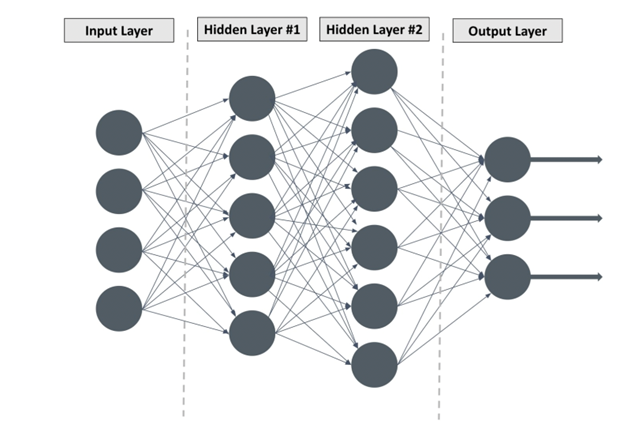
\includegraphics[width=0.6\textwidth]{Images/Layers}
	\caption{Layers in a Deep Neural Network \cite{Arne:2022}}
\end{figure}

The image above represents the workings of a deep neural network in a simple manner. The input layer is the layer on the left, while the output layer is the layer on the right. Because the values of the middle layers cannot be seen in the training set, they are known as hidden layers. Hidden layers are, to put it simply, calculated values that the network uses to perform its "magic." A network is deeper the more hidden layers there are between the input and output layers. Deep neural networks are often defined as ANNs with two or more hidden layers. Deep learning needs a lot of data to work well, but little human involvement. This is why employing deep networks is the best option for bigger datasets, such as collections of images of license plates. CNNs are a particular class of deep networks that work well for tackling image recognition issues. \cite{Lauzon:2012} 

\subsection{Convolution Neural Networks}
The Convolutional Neural Network is one of the most well-developed deep neural networks. The term “convolution” in Convolution Neural Network refers to the convolution linear mathematical operation between matrices. Convolutional, non-linear, pooling, and fully linked layers are among the many layers that make up CNN. Pooling and non-linearity layers lack parameters, but convolutional and fully connected layers do have them. \cite{Albawi:2017}  CNNs are incredibly helpful for identifying patterns in images that represent objects. For categorizing non-image data, such as audio, time series, and signal data, they can be highly useful. 

\begin{figure}[h!]
	\centering
	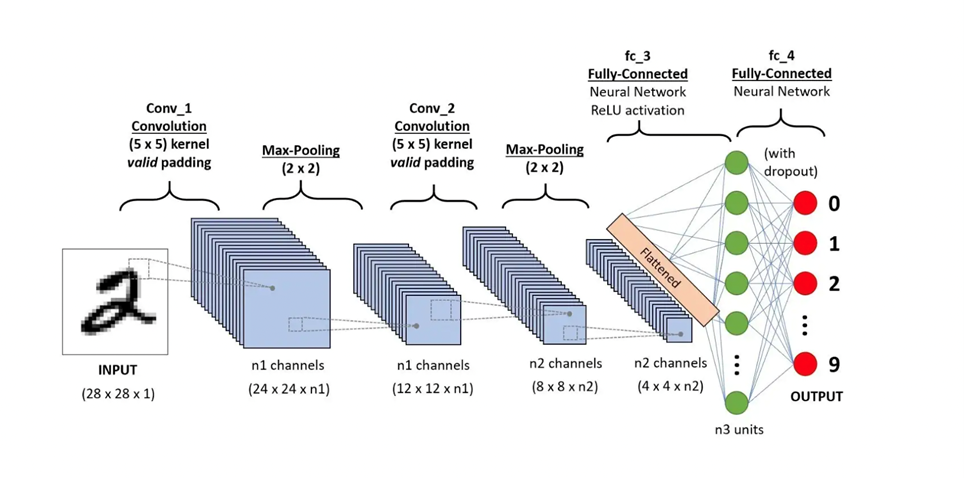
\includegraphics[width=\textwidth]{Images/CNNAp}
	\caption{Convolution neural network representation \cite{Chauhan:2018}}
\end{figure}

CNNs usually have 3 layers, a convolutional layer, a pooling layer and a fully connected layer. The first layer is used for feature extraction and for this a filter is used. The next layer is the pooling layer. This layer's main goal is to scale down the convolved feature map in order to save on computation expenses. By reducing the connections between layers and working separately on each feature map, this is accomplished. \cite{Chauhan:2018} There are various sorts of pooling operations, depending on the mechanism utilized. Max pooling and average pooling are available. To connect the neurons between two layers, the Fully Connected (FC) layer, which also includes weights and biases, is utilized. These layers make up the final few layers of a CNN architecture and are often positioned before the output layer. A neuron's activation status is determined by an activation function. As a result, it will determine whether or not the neuron's input to the network is crucial for prediction. The ReLU, Softmax, tanH, and Sigmoid functions are a few examples of regularly used activation functions. \cite{Chauhan:2018}

The challenge of image recognition and detection is a well-known one in machine learning. Finding an object in a digital image or video, or identifying an image therein, is an extremely difficult task. Face recognition, biometric systems, self-driving cars, emotion detection, picture restoration, robotics, and many more areas of computer vision are just a few of the computer vision fields where image recognition has applications. \cite{Chauhan:2018} The field of computer vision has made significant progress thanks to deep learning methods. To replicate the operations of the human cerebral cortex, deep learning uses artificial neural networks with numerous hidden layers. Deep neural network layers extract various features, offering several levels of abstraction as a result. With the ability to handle millions of parameters and reduce processing costs, convolutional neural networks take a 2D image as input, apply filters and kernels to it, and then output volumes. \cite{Chauhan:2018}
